\title{On the Path to Seamless Python Serverless Data Analytics}

\begin{abstract}
Before the rise of serverless computing, most data scientists relied heavily on traditional clusters of virtual machines to handle large-scale workloads. While these clusters were effective, they entailed substantial operational and maintenance costs, alongside increasing complexity in configuration and scaling — often demanding dedicated infrastructure specialists.

The serverless paradigm introduces a radically different model, centered on functions with automatic scaling and pay-per-use billing. To enable data analytics on serverless architectures, Lithops emerges as a powerful Python framework that abstracts away infrastructure complexities, empowering seamless parallel execution through serverless functions and allowing users to focus purely on their code.

A persistent challenge in serverless data analytics is the efficient partitioning of data, a crucial factor for maximizing parallelism and minimizing latency in data transfer from storage to compute resources. Dataplug addresses this by offering an on-the-fly partitioner that supports standard data formats, optimizing data extraction and distribution with precision.

To further streamline the scientific development experience, Pyrun tackles the steep learning curve posed by configuring and managing serverless environments for users without DevOps expertise. By providing a shared, remote browser-based environment seamlessly connected to the cloud provider, Pyrun drastically reduces the cognitive burden of setup — delivering a ready-to-execute environment with zero configuration required.

Ultimately, the integration of Lithops, Dataplug, and Pyrun forms a compelling stack that unlocks the full potential of serverless data analytics in Python, delivering clear and transformative benefits to modern scientific workflows.
\end{abstract}

\section{From Cluster-Centric to Serverless Data Analytics}
Data analytics has traditionally been conducted on clusters—networks of interconnected servers collaboratively processing and analyzing vast volumes of data. These clusters deliver the computational power, storage capacity, and parallelism necessary to address the growing scale and complexity of datasets across diverse domains such as finance, healthcare, and social media. By distributing workloads across multiple nodes, clusters enable efficient parallel execution, fault tolerance, and scalability, establishing themselves as the backbone of many big data frameworks like Apache Hadoop [] and Apache Spark []. The cluster-centric approach has proven effective for batch processing and iterative algorithms that demand high throughput and sustained computational resources.

Nonetheless, inherent limitations persist within this architecture for data analytics workloads. Resource overprovisioning is commonplace [], resulting in suboptimal and inefficient utilization. This inefficiency is particularly pronounced in scenarios with infrequent analytics executions, where users maintain clusters in a ready state without active workloads queued. Scalability also remains a critical challenge: server provisioning and deprovisioning often incur latencies of several minutes [], underscoring limited resource elasticity. Furthermore, the operational complexity and maintenance overhead of cluster-based frameworks such as Spark and Hadoop necessitate specialized expertise to configure, optimize, and sustain the computing environment.

Conversely, simpler computing models have emerged, notably with the introduction of Function-as-a-Service (FaaS) by AWS in 2014. This paradigm abstracts infrastructure management entirely, allowing developers to focus solely on their application logic. Additional advantages—including a pay-as-you-go pricing model and low invocation latencies—have sparked significant interest within the scientific community. While FaaS was not originally designed with data analytics workloads in mind, its potential for scalable, event-driven computation has motivated investigations into its viability as a core engine for distributed data analytics applications.

\section{Lithops: The Pythonic Serverless Data Analytics Framework}
Despite the previous suggested potential, leveraging FaaS platforms for large-scale data analytics presents several inherent challenges. These include the lack of direct peer-to-peer communication between functions, the absence of native synchronization mechanisms between stages (like in a MapReduce model), difficulties in managing dependencies and libraries across different cloud environments, and a general lack of portability due to proprietary APIs. Existing solutions have only partially addressed these issues; for instance, some frameworks facilitate communication but lack a simple programming model, while others are platform-specific.

To overcome these limitations comprehensively, Lithops [9] entered to scene, It is a serverless, multi-cloud framework designed for building both embarrassingly parallel and MapReduce-like applications using cloud functions. Lithops empowers users, even those without extensive cloud expertise, to effortlessly port their everyday programs—such as Monte Carlo simulations or sentiment analysis—to the cloud. By transparently orchestrating hundreds of concurrent function instances, Lithops enables significant performance gains for "occasional" cloud users who might otherwise be daunted by the complexities of cluster resource provisioning.

Specifically, Lithops addresses the aforementioned challenges by implementing a simple MapReduce interface that allows single-machine Python code to be executed as parallel jobs in the cloud. It also includes an intuitive storage API to facilitate communication between functions and with the Lithops client. Synchronization between map and reduce stages, including nested function compositions, is handled implicitly, reducing user burden, and Lithops automatically manages dependencies by leveraging Python's dynamic nature. Finally, its architecture is designed to abstract away cloud provider specifics, ensuring multi-cloud portability and mitigating vendor lock-in across platforms like IBM Cloud, Google Cloud, and AWS.

In essence, Lithops provides a unified system to leverage cloud functions for massively-parallel execution of ordinary programs, enabling hundreds-way parallelism on short-lived functions and significantly accelerating scientific and everyday computing tasks. 
%The source code for Lithops is openly available on its GitHub repository [9].

\subsection{Architecture}
The core design of Lithops is centered around abstracting the complexities of cloud functions and providers to offer a seamless experience for parallel program execution. At its heart, Lithops operates as a multi-cloud framework, capable of deploying and managing functions across various popular FaaS platforms, including AWS Lambda, IBM Cloud Functions, Google Cloud Functions, and Knative. This multi-cloud capability is a fundamental architectural choice aimed at mitigating vendor lock-in and offering users flexibility.

The architecture is built to facilitate massively-parallel execution of ordinary Python programs. Instead of requiring a persistent, warm cluster, Lithops is designed for short provisioning times, enabling the rapid spawning of hundreds or even thousands of cloud functions to execute large jobs within seconds. This dynamism is crucial for "occasional" users who benefit from on-demand parallelism without the overhead of continuous resource management.

Key architectural features include:

% add lithops_arch.png
\begin{figure}[htbp]
\centering
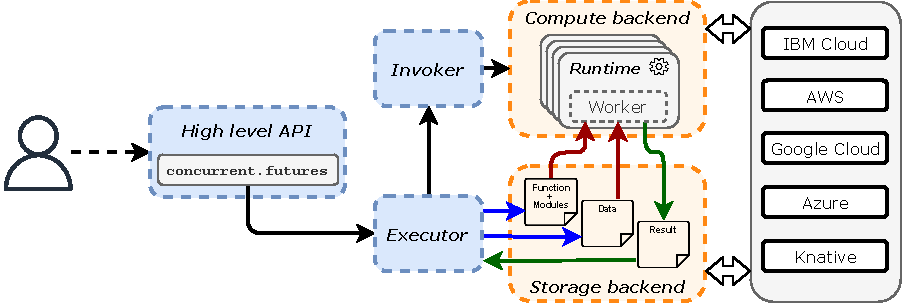
\includegraphics[width=\textwidth]{assets/lithops-scipy.pdf}
\caption{Lithops Architecture Overview}
\label{fig:lithops_arch}
\end{figure}

\begin{lstlisting}[language=Python, basicstyle=\ttfamily\small, commentstyle=\color{gray}]
"""
Simple Lithops example using the map() call to estimate PI
"""
import lithops
import random

def is_inside(n):
    count = 0
    for i in range(n):
        x = random.random()
        y = random.random()
        if x*x + y*y < 1:
            count += 1
    return count

if __name__ == '__main__':
    np, n = 10, 15000000
    part_count = [int(n/np)] * np
    fexec = lithops.FunctionExecutor()
    fexec.map(is_inside, part_count)
    results = fexec.get_result()
    pi = sum(results)/n*4
    print("Esitmated Pi: {}".format(pi))
\end{lstlisting}


\begin{itemize}
\item \textbf{Decoupled Execution and Storage}: Lithops leverages object storage services (e.g., S3, IBM Cloud Object Storage, Google Cloud Storage) as the primary mechanism for inter-function communication and data exchange. This design choice addresses the FaaS limitation of direct peer-to-peer communication, as functions can write to and read from shared storage buckets.
\item \textbf{Client-side Orchestration}: The Lithops client, typically running on a local machine (e.g., within a Jupyter notebook), orchestrates the parallel execution. It manages the partitioning of data, the launching of cloud functions, the loading of dependencies, and the collection of results.
\item \textbf{Dependency Handling}: The architecture incorporates mechanisms to automatically handle dependencies required by the user's Python code within the cloud function environment. This is achieved by exploiting the dynamism of the Python language, ensuring that the necessary libraries and modules are available to the ephemeral function instances.
\item \textbf{Implicit Synchronization}: The framework manages synchronization between different stages of a parallel computation (e.g., map and reduce phases) implicitly. This relieves the user from the tedious task of explicit synchronization, allowing them to focus on the application logic.
\end{itemize}

Overall, the Lithops architecture is a layered approach where the framework layer sits atop the serverless execution layer, addressing the unique restrictions of this brand-new computing environment by providing a unified and abstracted interface for massively-parallel computing.


\subsection{Programming Model}
Lithops provides a simplistic yet powerful programming model that allows users to translate their single-machine Python code into massively parallel cloud-based executions. The primary goal of this model is to significantly lower the barrier for users to leverage cloud FaaS platforms for parallel workloads, particularly those that exhibit innate parallelism, akin to the MapReduce paradigm.

The central component of the Lithops programming model is the \texttt{map()} primitive. Inspired by functional programming concepts and familiar to many Python developers, the \texttt{map()} primitive allows users to effortlessly spawn numerous concurrent function instances. By invoking \texttt{map()} on a function with a collection of inputs, Lithops transparently distributes the execution of that function across hundreds or thousands of cloud functions in the cloud. This enables users to:

\begin{itemize}
\item \textbf{Outsource "everyday" programs}: Users can take their existing Python scripts designed for single-machine execution (e.g., Monte Carlo simulations, sentiment analysis, hyper-parameter tuning) and, with minimal modifications, execute them in parallel on FaaS platforms.
\item \textbf{Leverage MapReduce-like patterns}: While providing a simple \texttt{map()} interface, Lithops implicitly supports the entire MapReduce computational pattern. This includes the ability to perform a "reduce" operation on the results of the map stage, with synchronization between these stages being automatically handled by the framework.
\item \textbf{Focus on application logic}: The programming model abstracts away the complexities of distributed computing, such as managing virtual machines, setting up clusters, handling network communication, or dealing with low-level cloud APIs. Users simply provide their function logic and data, and Lithops handles the parallelization and execution details.
\item \textbf{Seamless data handling}: Complementing the \texttt{map()} primitive is an intuitive storage API. This API allows functions to easily communicate with one another and with the Lithops client by reading and writing data to object storage, effectively replacing direct peer-to-peer communication with a shared, high-throughput storage layer.
\end{itemize}

The design philosophy behind the Lithops programming model is to offer a familiar and accessible interface for parallelism, making massive-scale cloud computing available to a broader range of users, including those without specialized distributed systems knowledge. This allows researchers and practitioners to quickly experiment with and deploy parallel analytics applications without significant upfront investment in learning complex cloud-specific programming paradigms.

\subsection{High-Performance Data Analytics}
Lithops is particularly well-suited for high-performance parallel data analytics tasks, enabling users to execute large-scale computations with minimal effort. By leveraging the \texttt{map()} primitive, users can distribute their data processing tasks across numerous cloud functions.

\textbf{*** 80GB aggregated bandwidth ***}

\textbf{*** comparison with traditional cluster startups ***}

\textbf{*** 1000 parallel functions started in less than 3 seconds ***}

\begin{figure}[htbp]
\centering
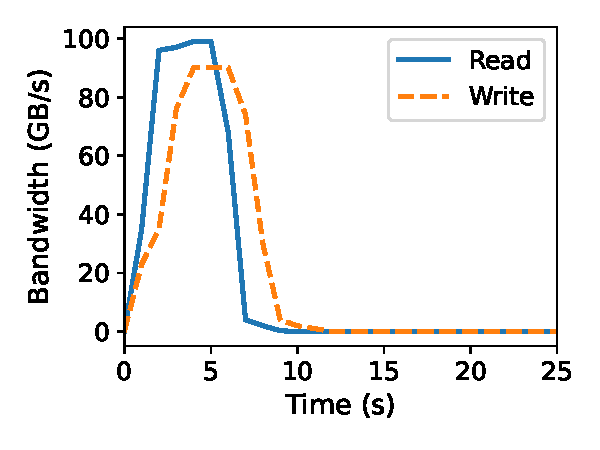
\includegraphics[width=0.7\textwidth]{assets/read_write.pdf}
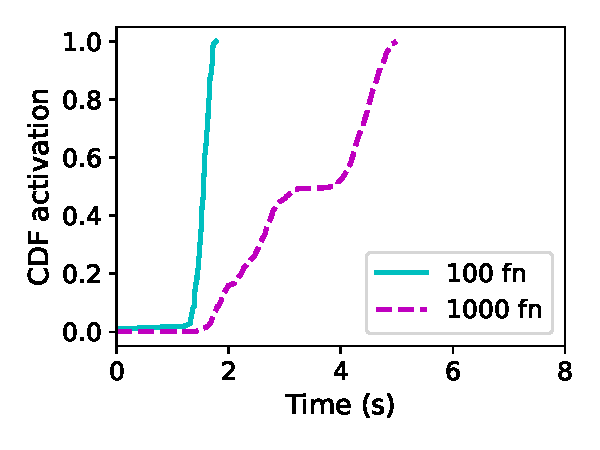
\includegraphics[width=0.7\textwidth]{assets/cdf_activation.pdf}
\caption{Lithops Performance: Latency and Throughput}
\label{fig:lithops_performance}
\end{figure}



\section{On the Road to On-the-Fly Partitioning}

Scientific computing in the cloud is becoming increasingly data-driven. The success of large-scale data-parallel workloads depends not only on scalable computation, but also on scalable data access. In this section, we examine the limitations of traditional data partitioning, introduce the concept of cloud-aware formats, and describe how the \texttt{Dataplug} framework enables dynamic on-the-fly partitioning of unstructured scientific data. We conclude with an overview of \texttt{Dataplug}'s three-stage workflow: \texttt{preprocess()}, \texttt{partition()}, and \texttt{get()}.

\subsection{The Static Partitioning Scenario}

Static data partitioning is a widespread strategy in scientific computing. It consists of physically splitting datasets into smaller chunks ahead of time, often based on size (e.g., 1~GB per file), and storing these chunks as individual objects. This enables distributed execution frameworks like Dask or Spark to process data in parallel by assigning each file to a separate worker.

While conceptually simple, static partitioning comes with significant limitations:

\begin{itemize}
    \item \textbf{High pre-processing cost}: Partitioning usually requires reading, transforming, and re-writing large datasets back to storage. In cloud object storage, where data is immutable, this implies full data duplication, leading to high I/O, storage, and compute costs.
    \item \textbf{Inflexibility}: Once partitioned, the chunk size is fixed. Adapting to new workloads (e.g., smaller partitions for finer-grained parallelism or larger ones for fewer tasks) requires reprocessing and rewriting the dataset again.
    \item \textbf{Format-dependency}: Many scientific data formats---such as compressed genomics data or binary point clouds---cannot be split arbitrarily. Partitioning such formats often breaks file structure or corrupts the data.
\end{itemize}

These limitations become increasingly problematic as scientific datasets grow to the petabyte scale. In practice, many research teams cannot afford the cost of rewriting legacy datasets just to enable parallel access. Moreover, partitioning choices made early in a project may later hinder performance optimization, preventing effective use of scalable resources.

\subsection{Cloud-Aware Formats Approach}

One proposed solution to static partitioning is to adopt so-called \emph{cloud-optimized formats}. These are file formats specifically designed to support partial reads using HTTP range requests over object storage. Examples include Cloud-Optimized GeoTIFF (COG), Cloud-Optimized Point Cloud (COPC), and Zarr.

Cloud-optimized formats share three key characteristics:

\begin{enumerate}
    \item \textbf{Indexable structure}: Internal content is arranged in a predictable structure (e.g., tiles, chunks, nodes).
    \item \textbf{Embedded metadata}: Indexing and partitioning information is stored inside the file itself, often in extended headers.
    \item \textbf{Compatibility with HTTP range access}: Chunks can be requested individually from object storage, allowing partial reads by distributed workers.
\end{enumerate}

While effective, this approach has its own challenges. Converting existing datasets to cloud-optimized formats requires a full rewrite of the data, which can be prohibitively expensive for large-scale archives. Moreover, not all scientific formats support reordering or embedding metadata---for example, text-based genomic formats like FASTQ or compressed binary LAS files for LiDAR data.

An alternative is \emph{retrofitting} cloud-awareness to legacy formats. Tools like \texttt{Kerchunk} allow generating external indexes for array formats (e.g., NetCDF, HDF5), enabling access through Zarr-compatible APIs. However, this is still limited to array-oriented structures and excludes many domain-specific formats used in genomics, metabolomics, and geospatial sciences.

\subsection{Dataplug: Enabling Dynamic Partitioning in Non-Cloud-Aware Formats}

\texttt{Dataplug} is a Python framework that implements a novel model: \emph{cloud-aware, on-the-fly dynamic partitioning}. The key idea is to separate indexing from data transformation. Rather than rewriting the data into a new format, \texttt{Dataplug} extracts structural metadata from the raw files via read-only pre-processing and stores this information externally (e.g., in a database or a metadata bucket). This enables parallel access to the original object without modifying it.

There are three essential building blocks:

\begin{itemize}
    \item \textbf{Cloud-aware pre-processing}: Each supported format defines a \texttt{preprocess()} function that analyzes the file structure (e.g., sequence boundaries, block offsets, spatial extents) and emits an index. This process is one-time and non-intrusive---it never rewrites the input data. For example, for compressed FASTQGZip files, the preprocessor uses \texttt{gztool} to extract random-access entry points.
    
    \item \textbf{Partitioning strategies}: Once pre-processed, a dataset can be partitioned in multiple ways using user-defined strategies. A \texttt{partition()} function queries the index and defines logical partitions (called \emph{slices}). For instance, one strategy might divide genomic data into 1 million reads per slice, while another partitions LiDAR files by bounding box. These strategies are pluggable and workload-specific.
    
    \item \textbf{Lazily-evaluated slices}: Each slice represents a logical data partition. When a worker calls \texttt{get()} on a slice, the slice retrieves the corresponding byte ranges from object storage (using HTTP range requests), assembles and possibly decompresses the data in memory, and returns it for processing. This happens entirely at runtime, just-in-time for processing.
\end{itemize}

This approach offers several benefits:

\begin{itemize}
    \item \textbf{Zero-cost re-partitioning}: Because partitioning operates over metadata, the same dataset can be re-sliced on demand with different strategies, without re-reading or re-writing the raw data.
    \item \textbf{Efficient resource usage}: The metadata is lightweight (often $<1\%$ of the original file size), and slices can be distributed to any number of workers, enabling elastic autoscaling.
    \item \textbf{Format extensibility}: Support for new formats is added by implementing a preprocessor, a strategy, and a slice handler---no need to modify the core.
\end{itemize}

\subsection{The Main Loop: \texttt{preprocess()}, \texttt{partition()}, \texttt{get()}}

The \texttt{Dataplug} workflow can be summarized in three steps:

\begin{enumerate}
    \item \textbf{Preprocessing (\texttt{preprocess()})}: This step is done once per object. The user (or an automated trigger) calls \texttt{preprocess()} on a \texttt{CloudObject}, specifying the format (e.g., \texttt{FASTQGZip}). The system runs the corresponding logic to extract structural metadata and stores it externally.
    
    \item \textbf{Partitioning (\texttt{partition()})}: Once indexed, the user applies a partitioning strategy to generate slices. A call to \texttt{partition()} returns a list of lazy-evaluated \texttt{DataSlice} objects, each representing a logical chunk. These can then be submitted as input to any Python parallel execution framework (e.g., \texttt{ipyparallel}, \texttt{Ray}, \texttt{Dask Bag}, etc.).
    
    \item \textbf{Fetching (\texttt{get()})}: Inside the worker function, calling \texttt{slice.get()} retrieves and prepares the actual data partition from object storage. This includes issuing multiple concurrent byte-range requests, decompressing if needed, and returning a Python object (e.g., string, array, point cloud) ready for processing.
\end{enumerate}

\noindent Example usage:

\begin{lstlisting}[language=Python, basicstyle=\ttfamily\small, commentstyle=\color{gray}]
co = CloudObject.from_s3(FASTQGZip, 's3://bucket/sample.fastq.gz')
co.preprocess(AWSLambdaPreprocessor())
slices = co.partition(partition_num_reads, num_seq_partition=1_000_000)

def analyze(slice: FASTQGZipSlice):
    chunk = slice.get()
    return analyze_reads(chunk)

with ipyparallel.Cluster() as cluster:
    view = cluster.load_balanced_view()
    results = view.map(analyze, slices)
\end{lstlisting}

This model has been validated across diverse domains. For example:

\begin{itemize}
    \item \textbf{Genomics (FASTQGZip)}: Cloud-aware partitioning reduced pre-processing time by 65\%, avoided recompression, and enabled dynamic chunk-size tuning to optimize throughput and cost.
    \item \textbf{Geospatial (LiDAR LAS)}: Legacy LAS files were indexed with \texttt{lasindex}, enabling partitioning by region-of-interest without format conversion to COPC. This resulted in 71\% lower pre-processing time and better scalability on autoscaling clusters.
\end{itemize}


\begin{figure}[htbp]
\centering

\includegraphics[width=\textwidth]{assets/static-vs-dynamic.pdf}
\caption{Static and Dynamic partitioning approaches}
\label{fig:lithops_arch}
\end{figure}

\begin{figure}[htbp]
\centering
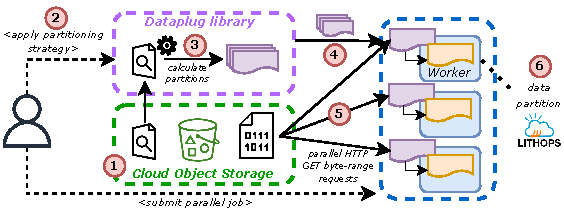
\includegraphics[width=\textwidth]{assets/dataplug.pdf}
\caption{Dataplug workflow}
\label{fig:lithops_arch}
\end{figure}

\section{Pyrun: Simplifying Serverless Environments for Data Science}

\begin{figure}[htbp]
\centering
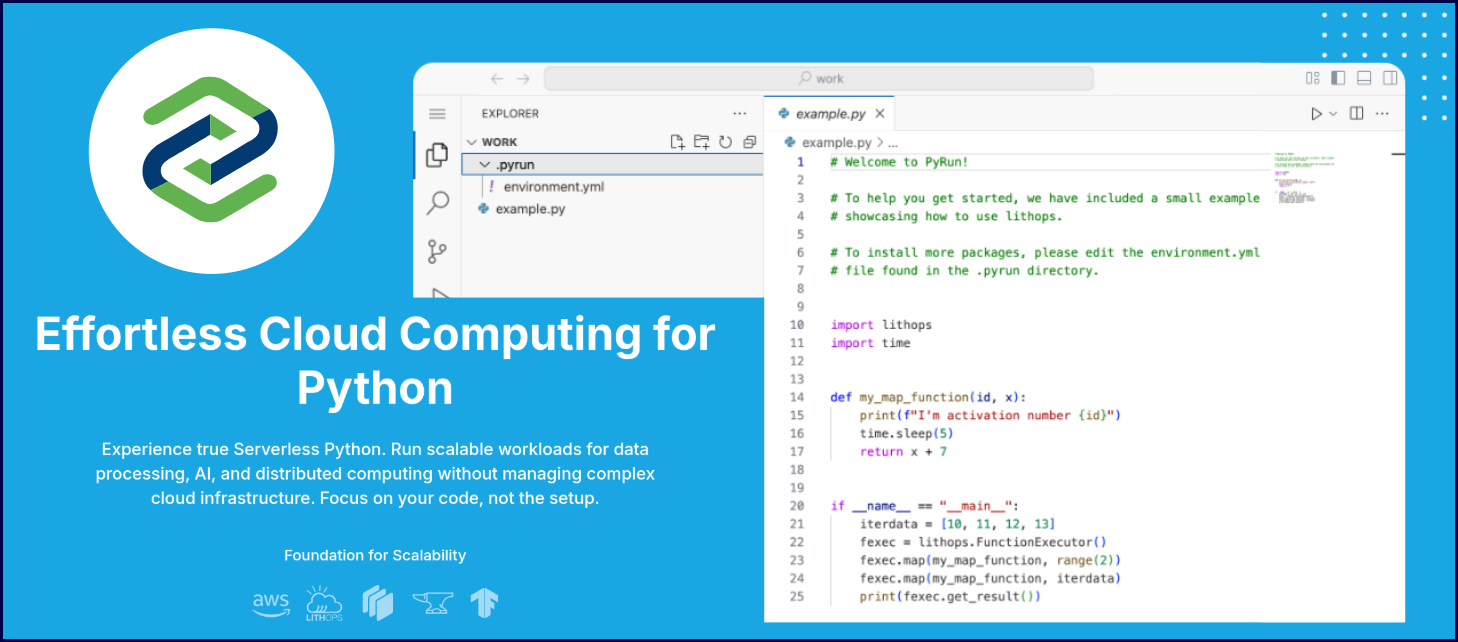
\includegraphics[width=\textwidth]{assets/pyrun.png}
\caption{PyRun.cloud}
\label{fig:lithops_arch}
\end{figure}

PyRun es un servicio en la nube que simplifica el desarrollo y la ejecución de aplicaciones serverless, especialmente en ciencia de datos y computación científica. Ofrece un entorno remoto y compartido, accesible desde el navegador, que elimina la necesidad de configurar o gestionar infraestructura, incluso para usuarios sin experiencia en DevOps. PyRun integra de forma nativa los frameworks Lithops y Dataplug, permitiendo ejecutar aplicaciones paralelas con un solo clic, sin preocuparse por la gestión de recursos en la nube. 

At a glance, tras linkar PyRun con nuestro proveedor cloud, the service offers the following features: 

\begin{itemize}

\item Ready-to-execute web-IDE: por cada una de las aplicaciones PyRun, tendremos un entorno remoto web-based, que nos brinda acceso via navegador al entorno de desarrollo. Además, el dev environment también se sincroniza nativamente con Github, permitiendo el ciclo de desarrolo sin necesidad de instalaciones adicionales. 

\item Pre-configured frameworks: hasta el momento, PyRun ya cuenta con integraciones de Lithops y Dataplug entre sus posibilidades, aunque en un futuro la lista de frameworks de computación paralela integrados crecerá. Estas integraciones permiten utilizar los frameworks de computación paralelas mediante sus APIs, pero sin la necesidad de realizar las tediosas preconfiguraciones, que suponen un paso más previo al desarrollo y/o ejecución.  

\item Sharing applications via Pipelines: Pyrun permite la compartición de aplicaciones paralelas via Public Resources, un espacio colaborativo donde los científicos de datos pueden abrir el acceso a sus aplicaciones, faciltando la cooperación entre la comunidad científica. 

\item Monitoring: PyRun se preocupa por la observabilidad de las aplicaciones paralelas científicas que se encargará de ejecutar. Es por ello por lo que pone a disposición de sus usuarios un espacio de monitoring, donde se mostrarán los datos de ejecución de las tareas subyacentes: estado de las tareas, consumo de CPU/memoria/red, funciones falladas, estadísticas de ejecución, etc. 

\item PyRun simplifies AI/ML workflows, allowing you to focus on model development by providing an integrated environment and automated management. It supports popular AI frameworks like TensorFlow and PyTorch with easy runtime configuration. You can achieve scalable data and training through Lithops for distributed processing. Additionally, PyRun offers interactive LLM environments, enabling local experimentation with models like Llama 3 via Ollama in your workspace. 
\end{itemize}

En resumen, PyRun.cloud es una plataforma que simplifica el desarrollo y la ejecución de aplicaciones serverless y AI/ML workflows. Para más información, puedes visitar su página web oficial: \url{https://pyrun.cloud/}.

\section{A Success Story in Python Serverless Data Analytics: METASPACE Metabolomics Pipeline}

\begin{figure}[htbp]
\centering
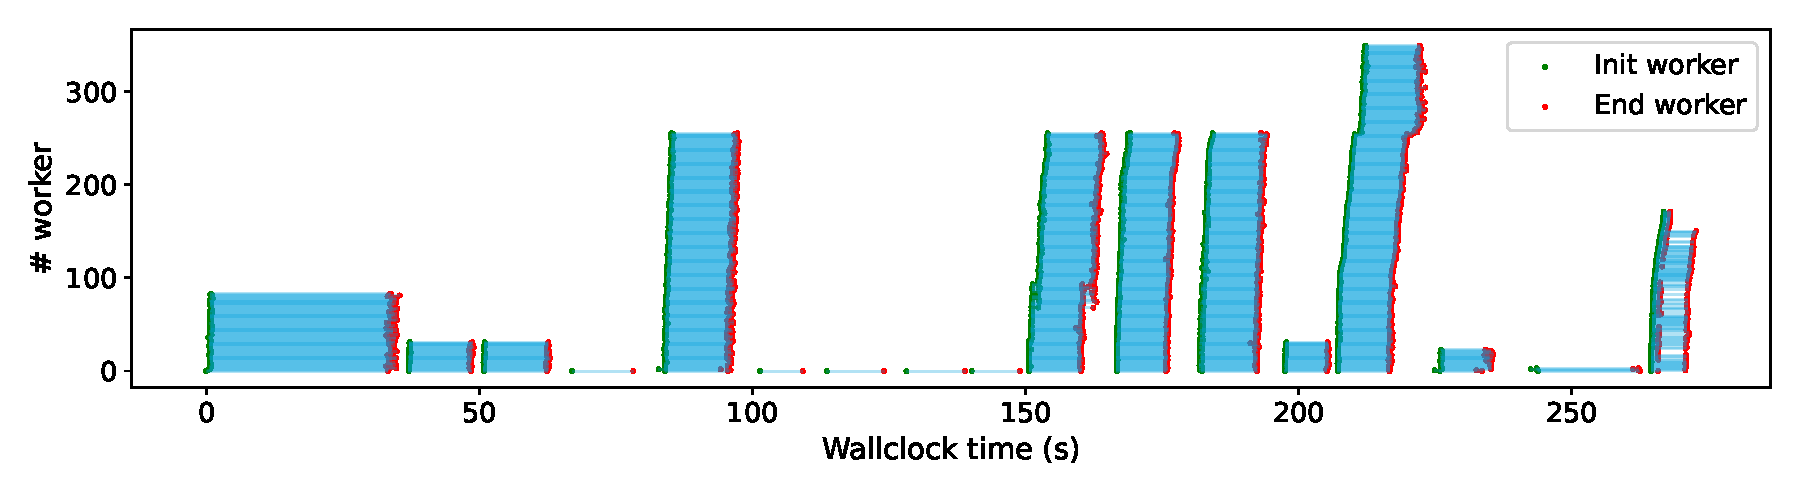
\includegraphics[width=\textwidth]{assets/wallclock.pdf}
\caption{METASPACE Metabolomics Pipeline}
\label{fig:lithops_arch}
\end{figure}

%\begin{figure}[htbp]
%\centering
%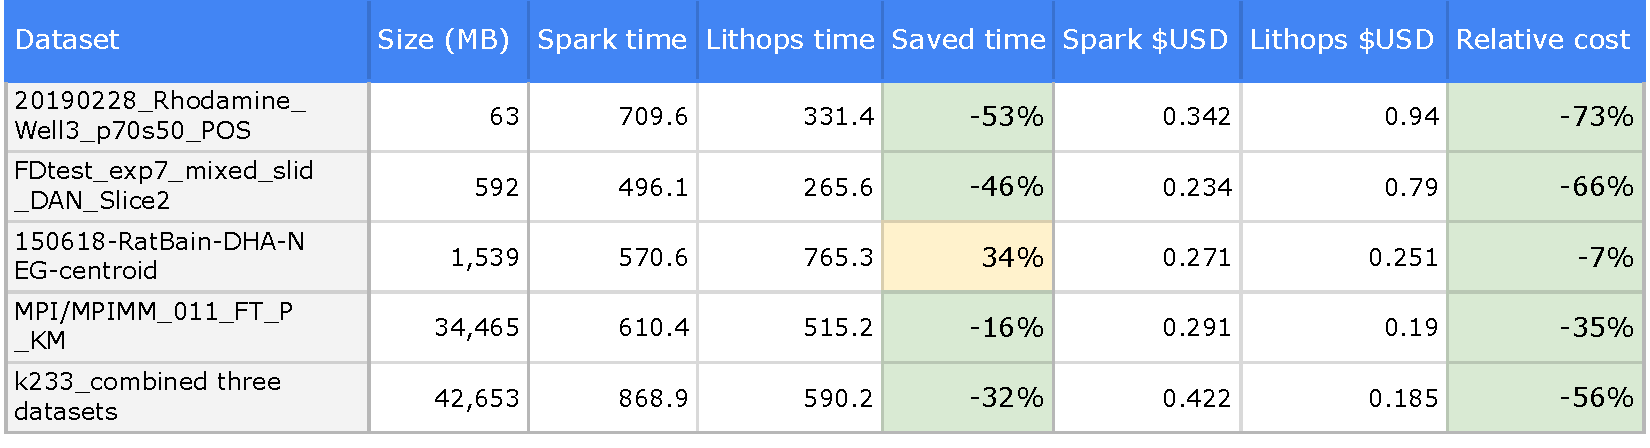
\includegraphics[width=\textwidth]{assets/table-meta.pdf}
%\caption{METASPACE Metabolomics Pipeline}
%\label{fig:lithops_arch}
%\end{figure}

\begin{figure}[htbp]
\centering
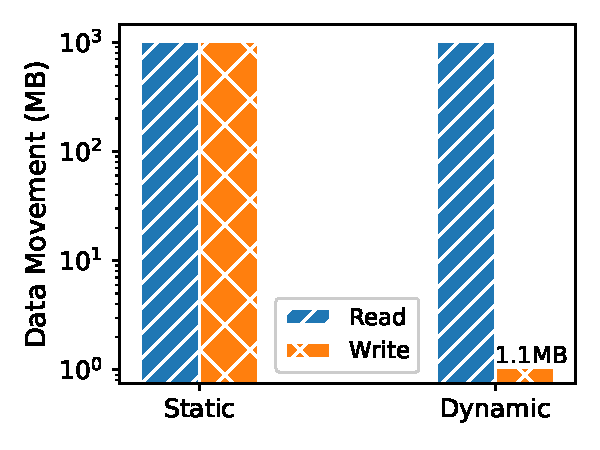
\includegraphics[width=0.675\textwidth]{assets/datamovement.pdf}
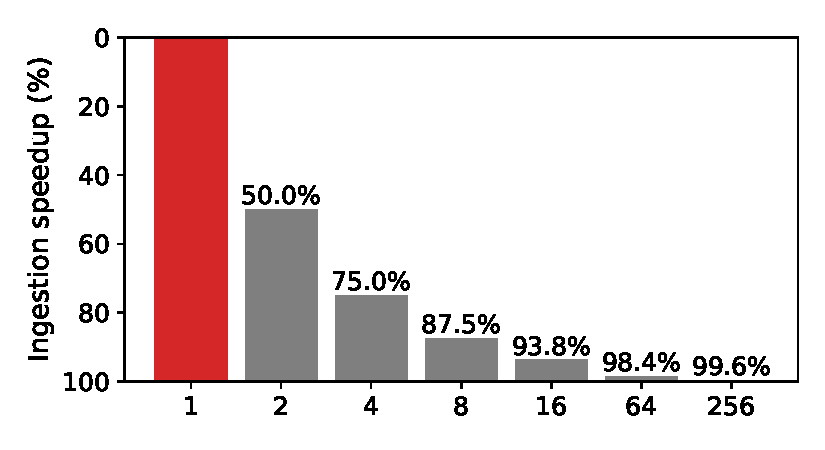
\includegraphics[width=1\textwidth]{assets/downloading.pdf}
\caption{Dataplug Performance: Preprocessing and ingestion}
\label{fig:dataplug_performance}
\end{figure}